% !TEX root = main.tex

\section{Motivation}

The widespread adoption of the web has emphasized the importance of ensuring that online content is accessible to everyone, including individuals with various disabilities\cite{abu2023web}. Despite this, less than 4\% of the top one million websites are fully accessible. Over 96\% contain detectable \ac{WCAG} failures, with an average of 51 errors per page \cite{webaimmillion2025}. Common issues include missing alt text (present on 56\% of home pages), low contrast, and poor form labeling \cite{audioeye2024}.

Meanwhile, the legal landscape is becoming stricter. The European Accessibility Act mandates compliance by June 28, 2025 for both public and private digital services in the EU, affecting more than 87 million EU residents with disabilities \cite{audioeyeEAA2025, accessibleEU2025}. % no se si poner este parrafo

On the other hand, rigorous testing is integral to ensuring reliability of web applications. For example, usability testing that involves having real users interacting with a live web application, allows for the identification of issues in action, enables for iterative feedback and a more realistic assessment of how they might experience the interface. Effective testing improves satisfaction, avoids rework, and ensures genuinely inclusive design \cite{accessdesign2025}.

Although \ac{WCAG} articulate extensive criteria for inclusive design \cite{w3c_WCAG22}, existing tools focus more on compliance than on realistic user behavior. Developers and UX practitioners often lack practical mechanisms to validate these guidelines in realistic usage scenarios. For instance, some of the significant challenges found in testing are little room for iteration, lack of extensive and appropiate user feedback, and limitations to empathy-based research methods\cite{lu2025uxagent}.


\section{Automated Testing}

Dynamic testing can help developers and stakeholders verify and validate that running software is working as expected. In this case, automated testing is the enabler for faster, more reliable and overall optimized testing. Automated testing leveraged by machine learning and \ac{AI} are increasingly becoming more popular and sophisticated, therefore using them in this scenario is a big step forward for ensuring accessibility. %aqui seria bueno poner una referencia de TSDL

Intelligent agents can interact with web content without access to the underlying code, relying instead on the same content the final user is interacting with\cite{lanham2025ai, wang2024survey, lu2025uxagent}. They can also be adapted based on feedback, and can process rich multimodal inputs, such as screenshots and screen reader text, enabling them to reason about both the visual layout and the spoken feedback of the user interface simultaneously. They are also able to use different interaction techniques, like keyboard only, mouse only, etc. This integrated perception allows for a more comprehensive assessment of accessibility issues that may arise during real user interactions. Finally, LLM agents excel at open-ended reasoning and can provide qualitative insights, alongside quantitative logs. However, they require careful prompting and can be slower or less predictable.


\section{Objectives}

First, we aim to explore the use of perceptual filters and multimodal inputs, such as applying blur to simulate different impairments; while also using screen reader outputs, to approximate the experience of real world users. 

Additionally, we will analyze whether certain UI elements become inaccessible or difficult to perceive under these simulated conditions, and investigate if common layout structures or design patterns can fail in these situations. Through this approach, we seek to identify not only the direct effects of visual filters on usability, but also the broader structural and behavioral implications for accessible web design.

\section{System design}
\subsection{Visual Filtering}

Simulating visual impairments through perceptual filters allows us to approximate the experiences of users with conditions such as glaucoma and myopia. These filters alter the rendered webpage in ways that reflect known physiological effects, such as peripheral vision loss, blur, or reduced contrast sensitivity.

\begin{figure}
    \centering
    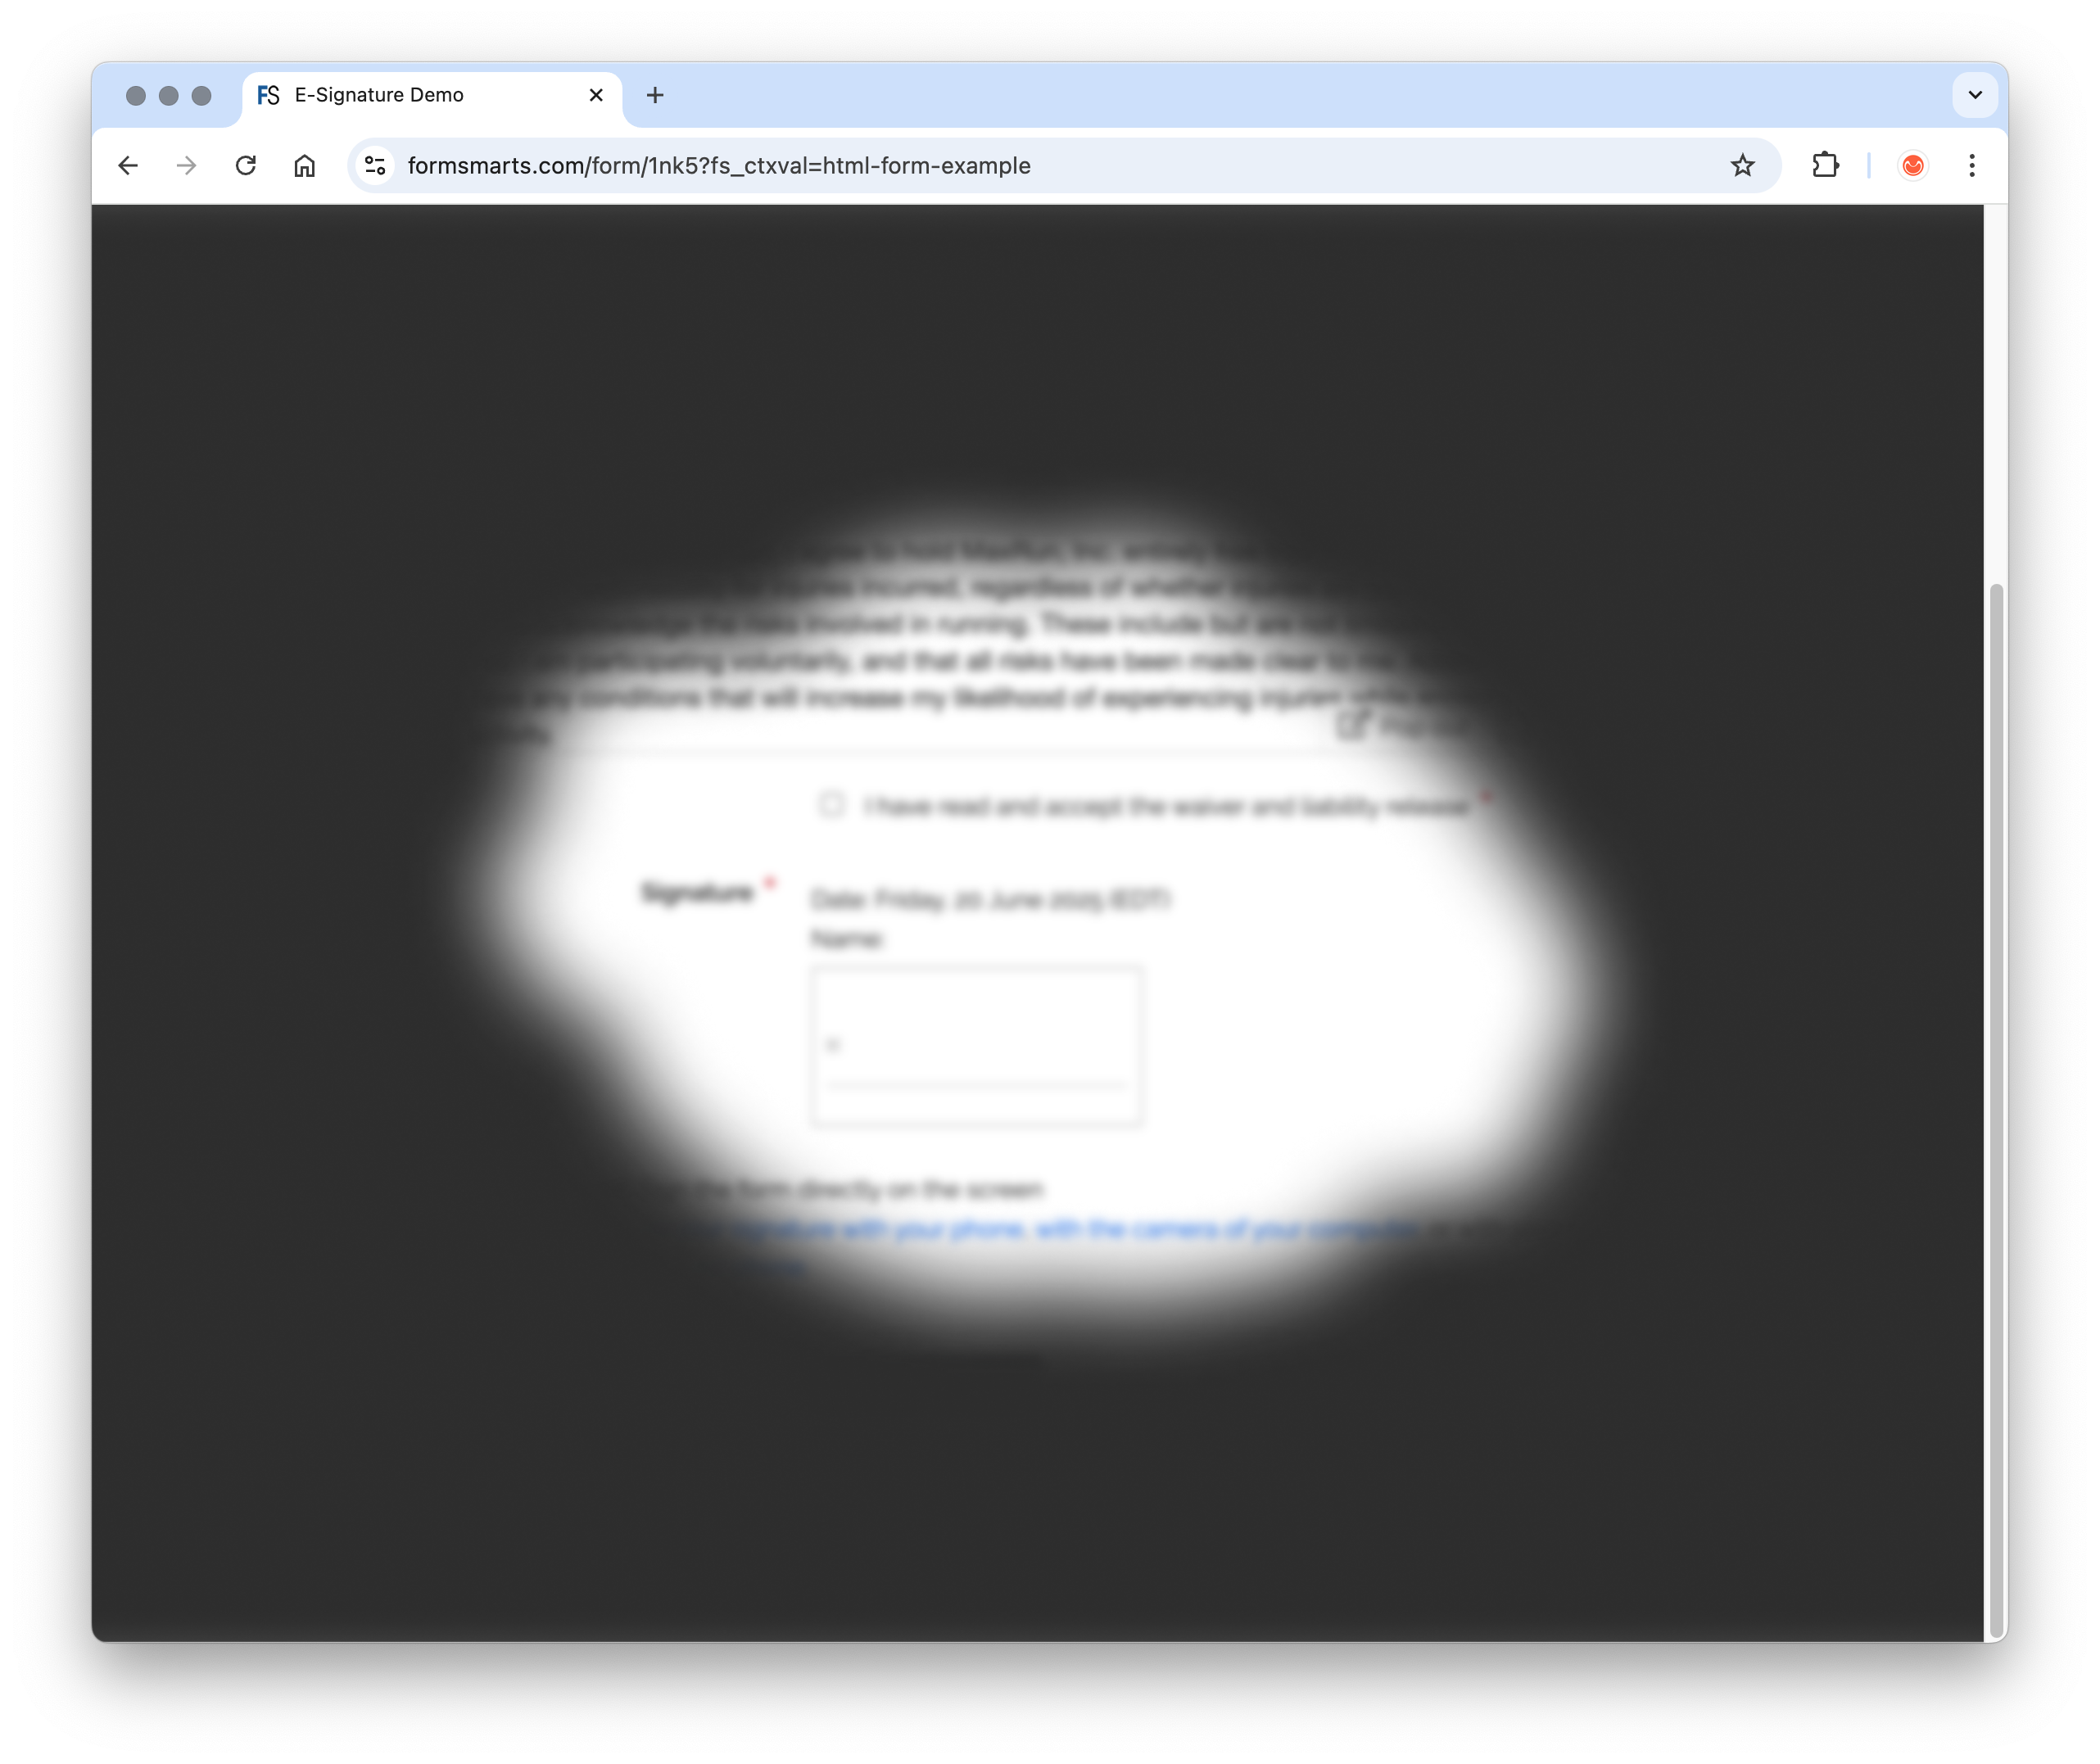
\includegraphics[width=115pt]{imgs/glaucoma-filter.png}
    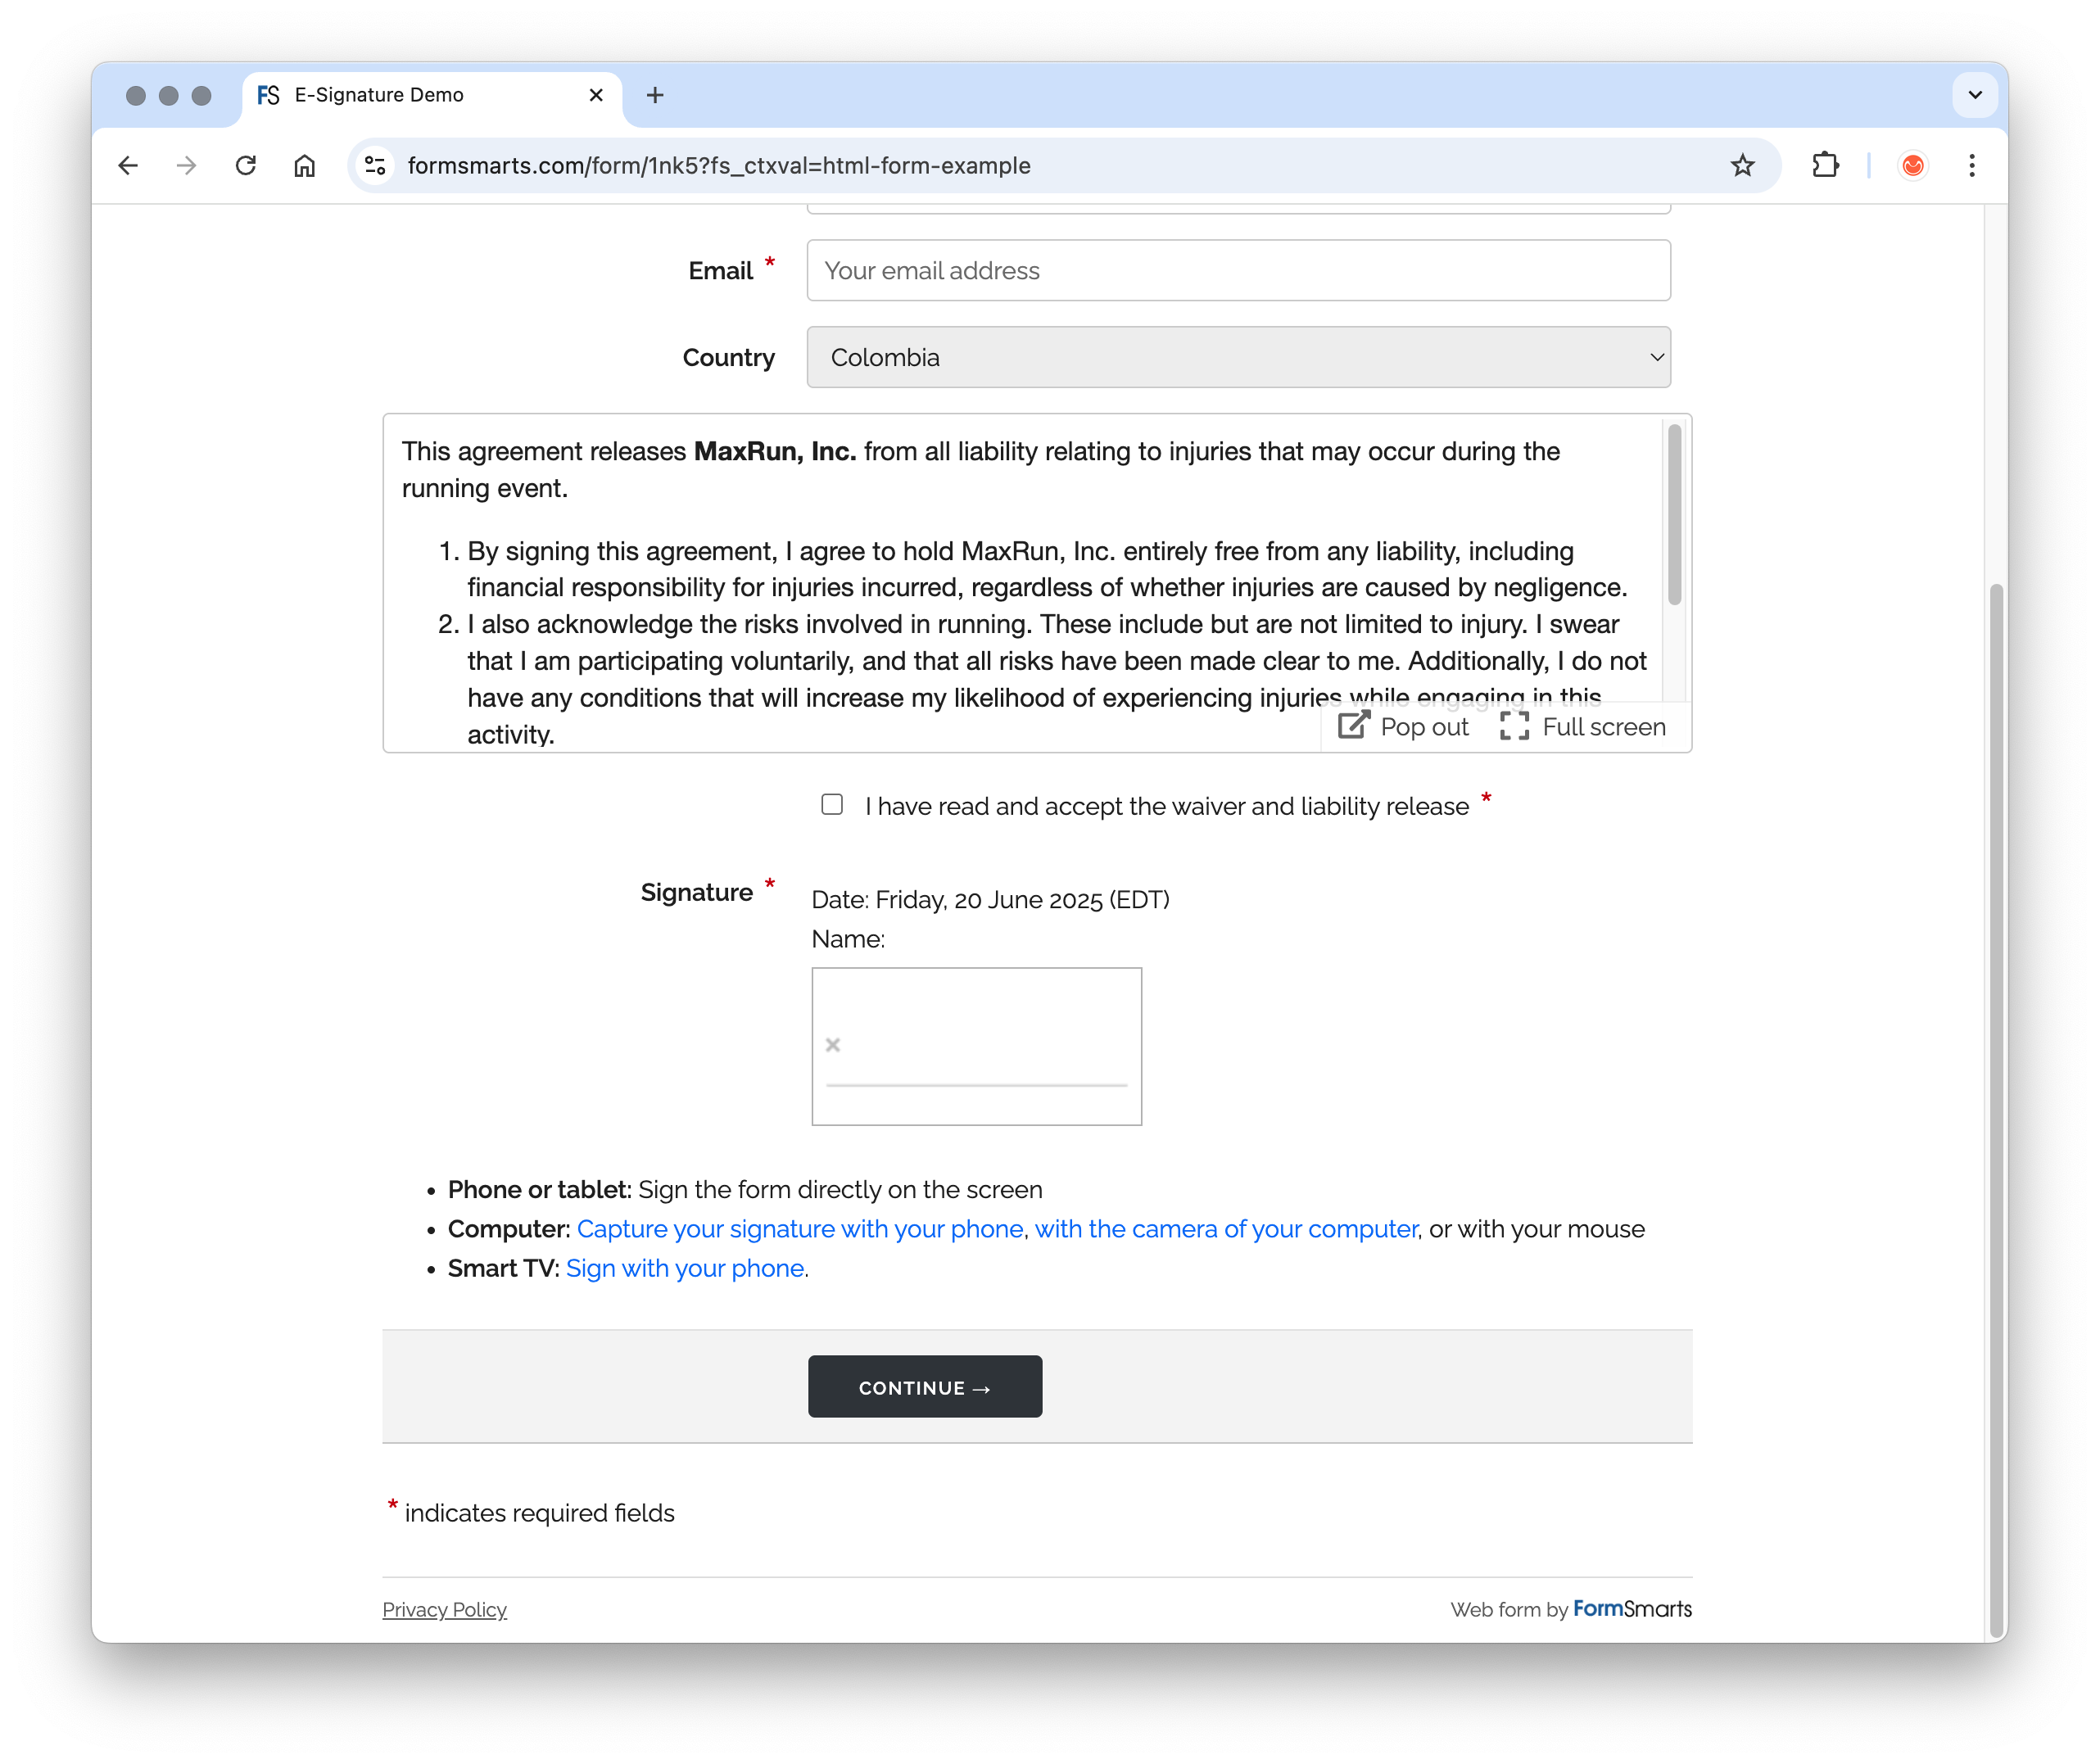
\includegraphics[width=115pt]{imgs/no-glaucoma-filter.png}
    \caption{Left: Glaucoma filter applied to an example form requiring a signature. The "Submit" button is no longer visible, making it difficult to locate. Right: Original version.}
    \label{fig:glaucoma-filters}
\end{figure}

\begin{figure}
    \centering
    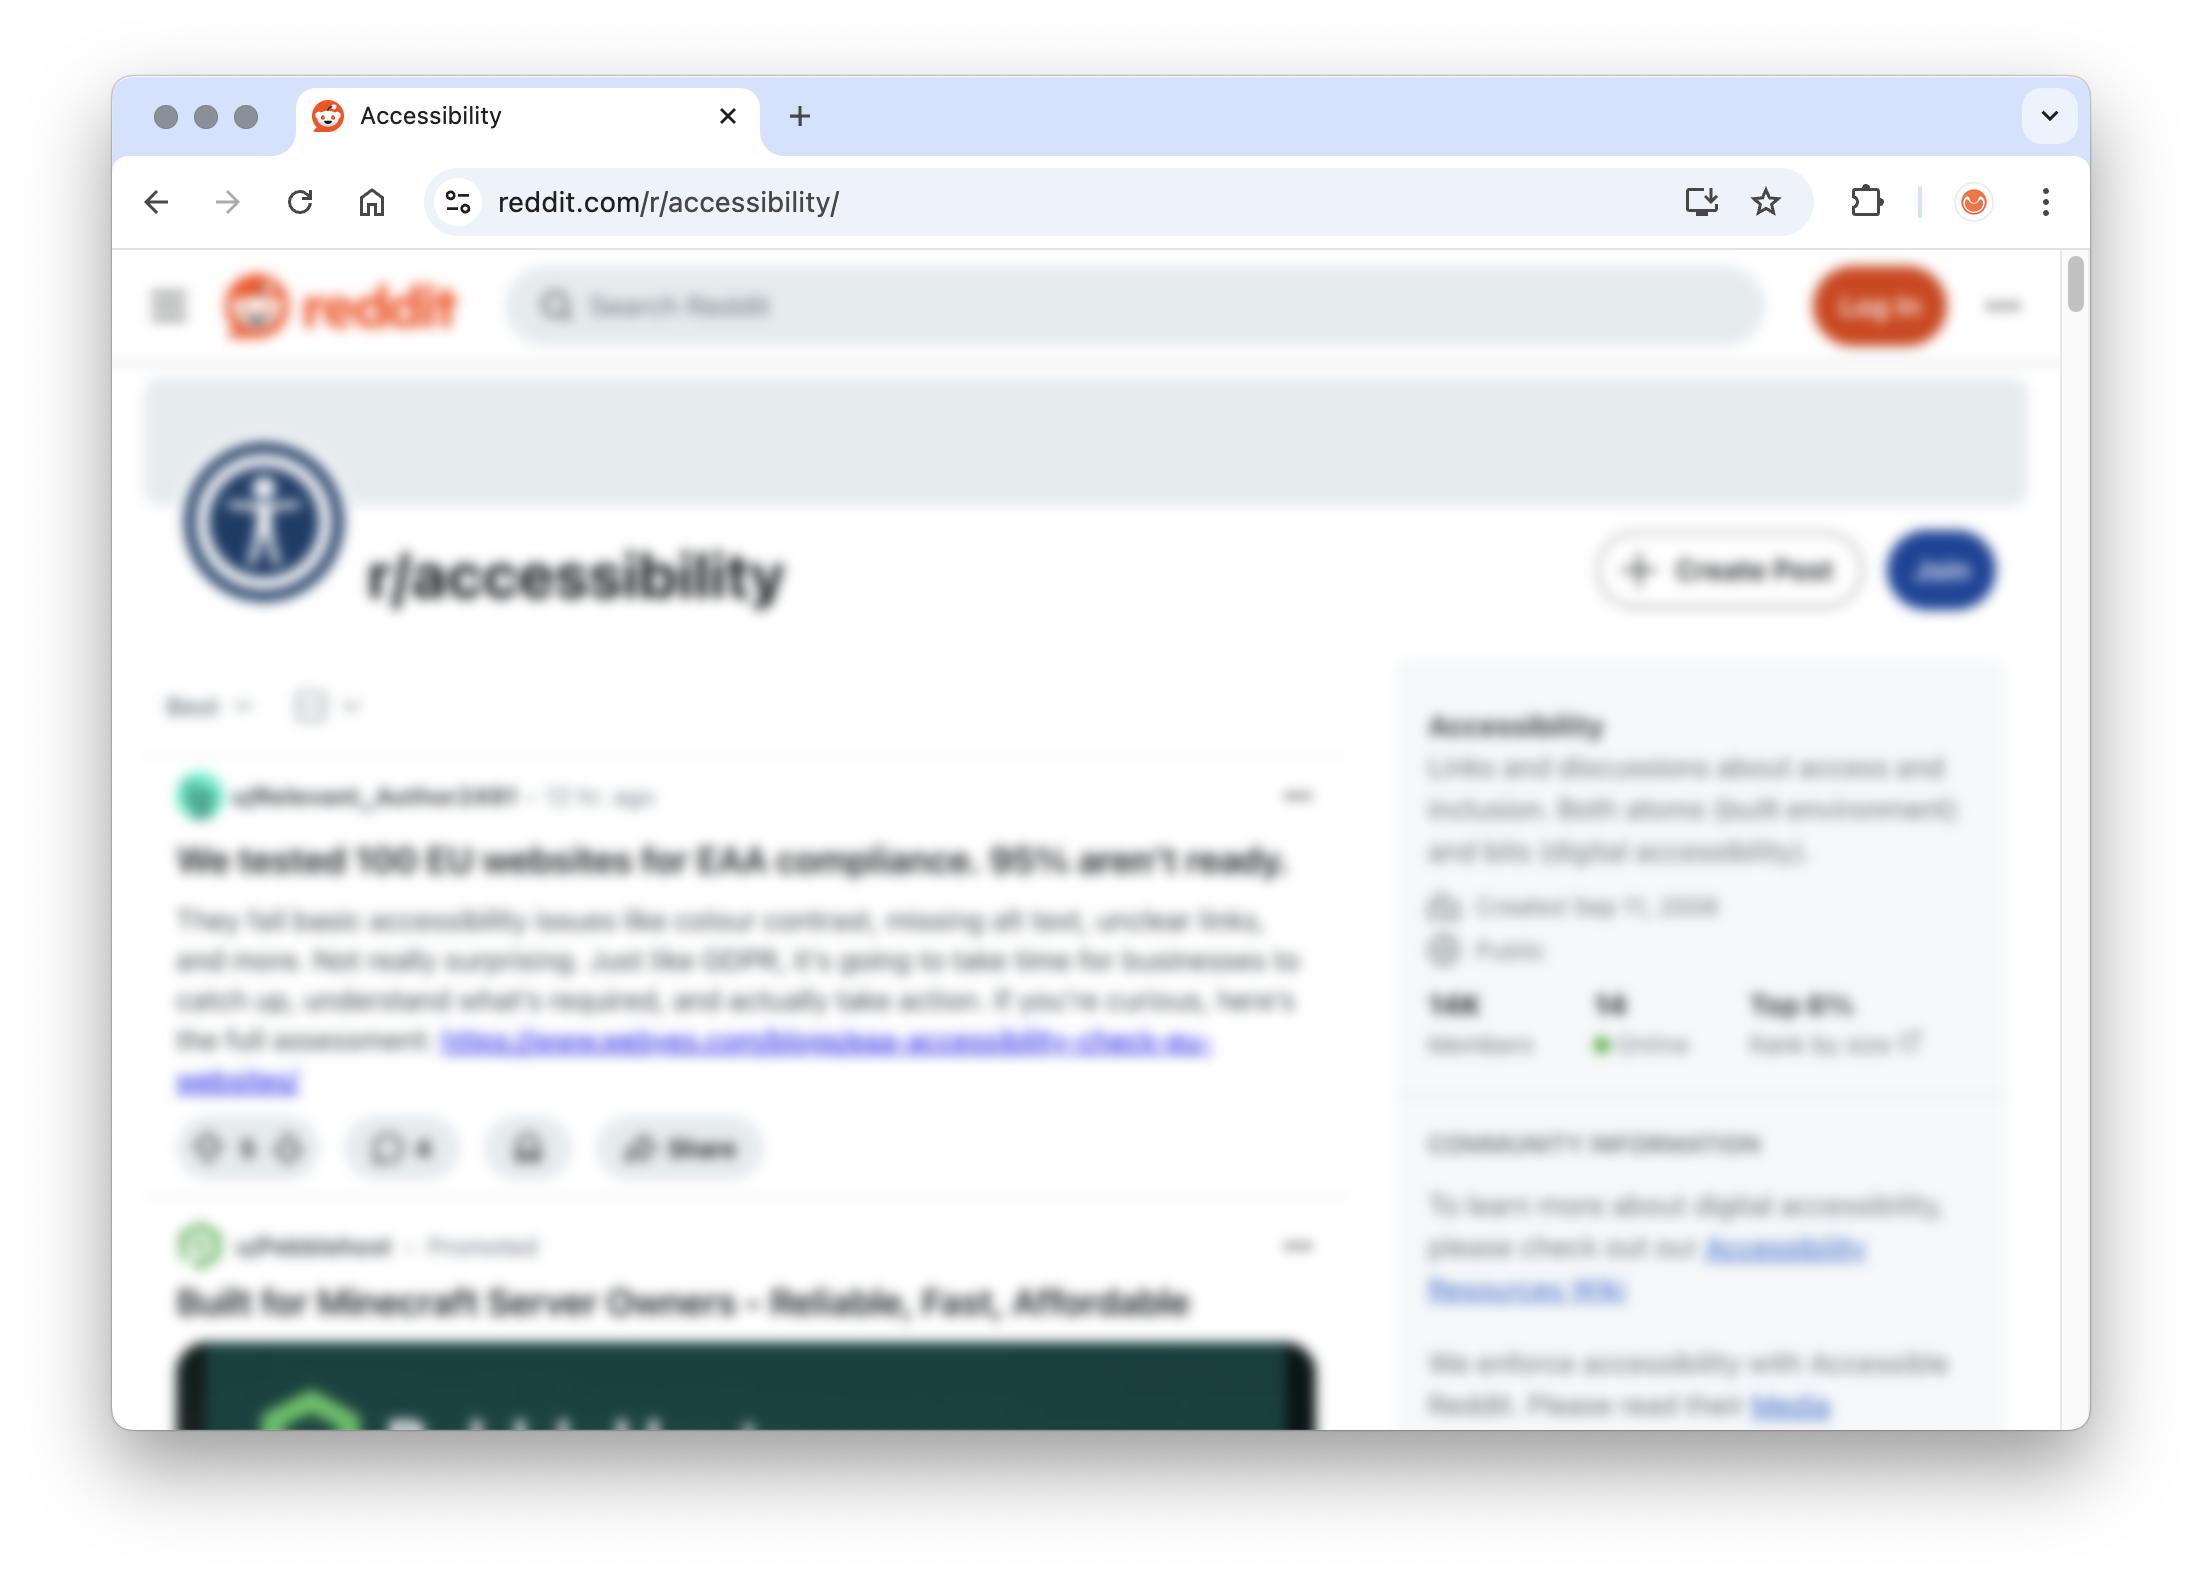
\includegraphics[width=115pt]{imgs/myopia-filter.png}
    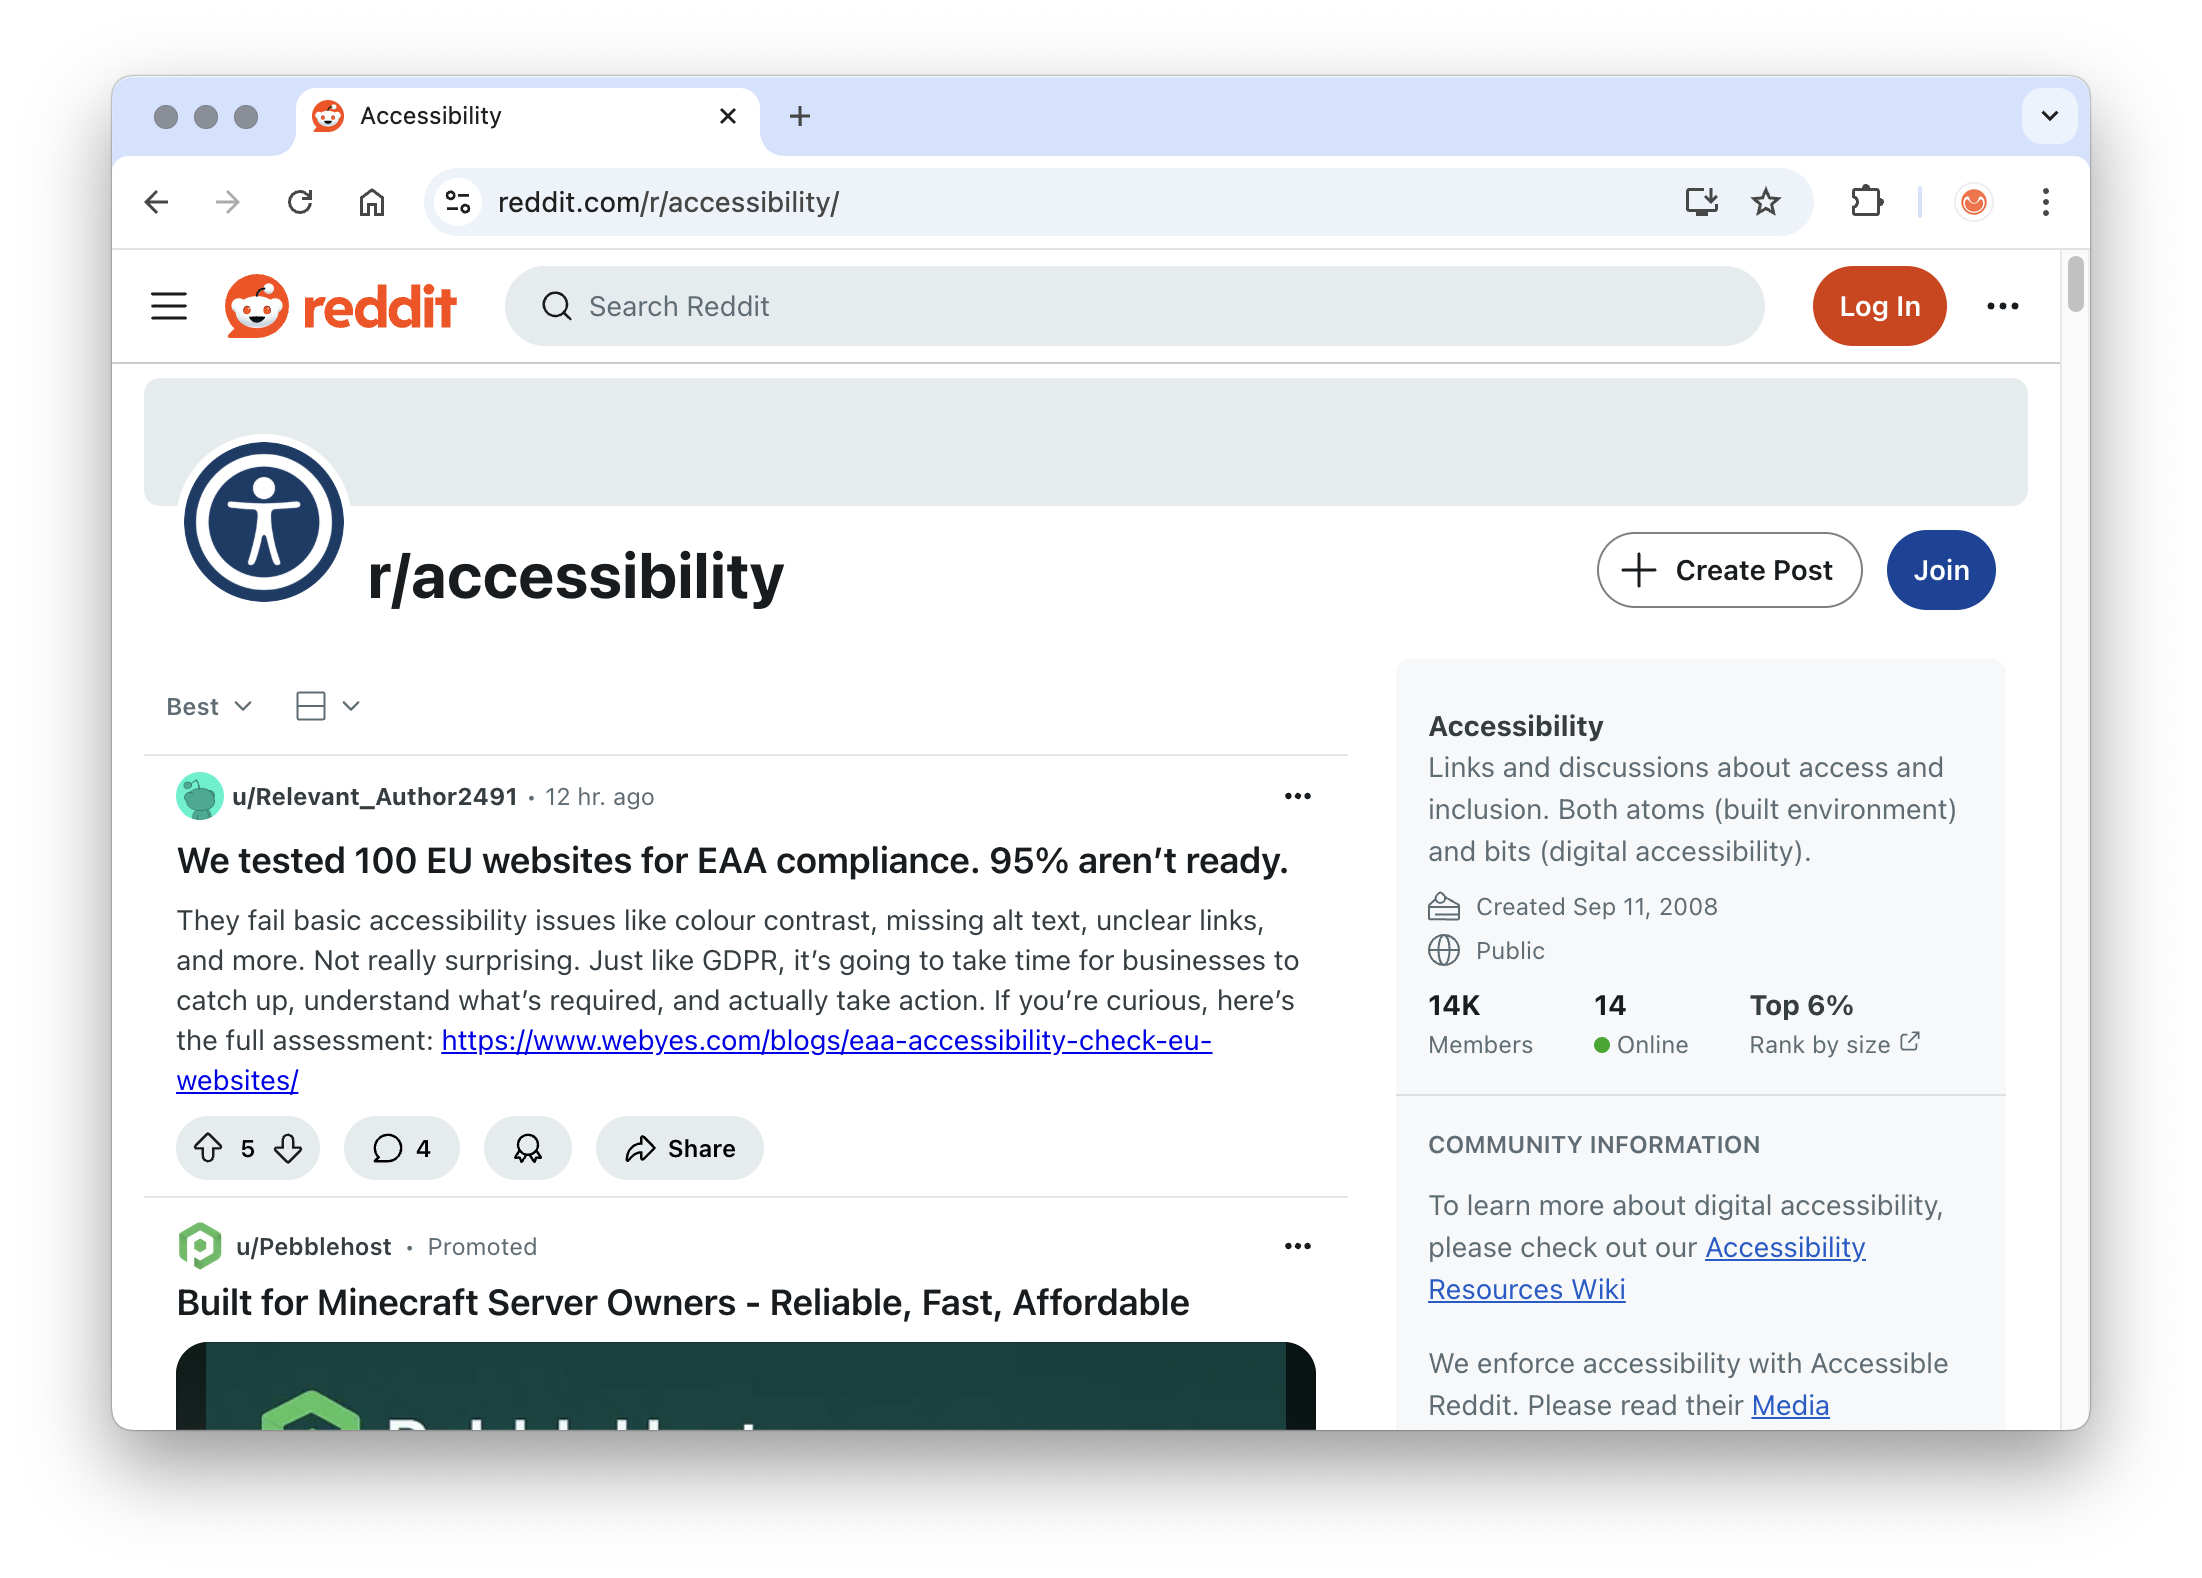
\includegraphics[width=115pt]{imgs/no-myopia-filter.png}
    \caption{Left: Myopia filter (-3 diopters) applied to a social media webpage, reducing clarity and edge sharpness. Right: Original version.}
    \label{fig:myopia-filters}
\end{figure}

These simulations (see figures. \ref{fig:glaucoma-filters} and \ref{fig:myopia-filters}) were implemented using the Visual Impairments Simulator Chrome extension \cite{visual_impairments_simulator}. While such tools provide a useful approximation of typical visual conditions, they are inherently limited: visual disabilities are highly individualized, and no filter can perfectly replicate the subjective visual experience of every user.

Future work should involve collaboration with ophthalmologists and vision science experts to improve the realism and clinical accuracy of these filters. Their insight can guide the calibration of filter parameters and help us design simulations that more closely resemble the lived experiences of users with specific visual conditions.

\subsection{Assistive output integration}

\begin{figure}
    \centering
    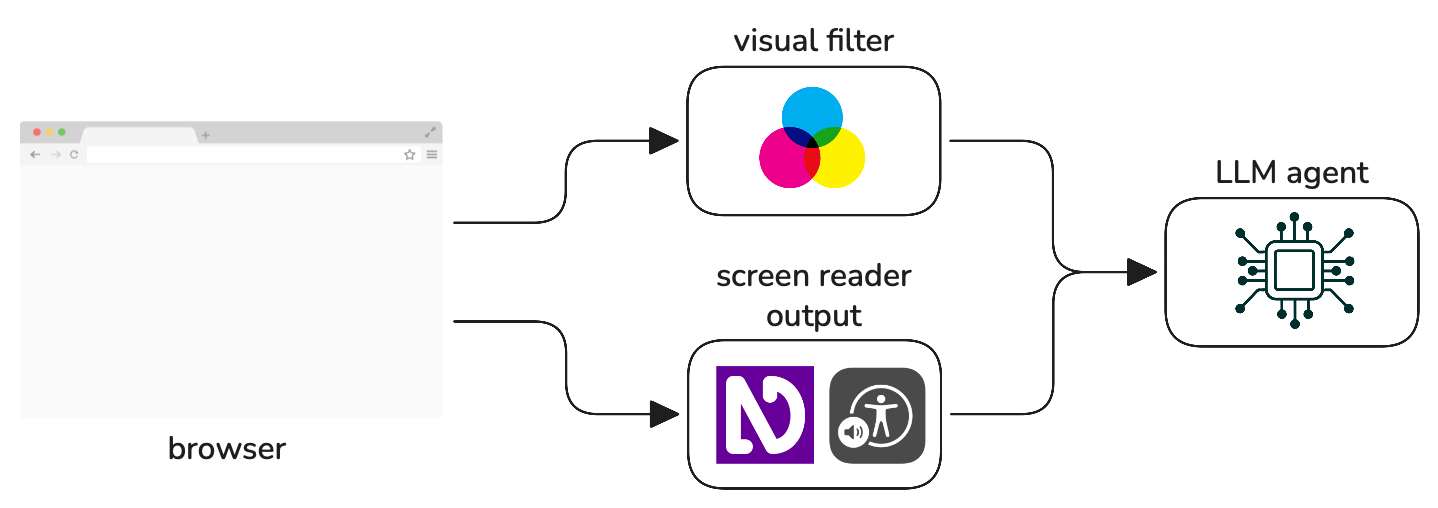
\includegraphics[width=1\linewidth]{imgs/flow.png}
\caption{Proposed pipeline for the agent feeding inputs}
\label{fig:pipeline}
\end{figure}


The agent must capture what an assistive technology user would hear and do. For screen reader output, we can integrate a driver API, such as Guidepup that programmatically controls VoiceOver (macOS) or NVDA (Windows). This driver issues the same keyboard commands a user would and exposes the spoken utterances\cite{guidepup2025}. The agent framework would invoke this API at each step and record the resulting stringof text (including element role, name, state) as sensory input.

For keyboard-only navigation logs, the agent can simply log focus events. As the agent presses Tab, arrow keys, Enter, etc., a browser automation framework, such as Playwright, Selenium or Kraken, can attach listeners to record each focus transition and action. This yields a sequence of elements visited in order\cite{ravelo2023kraken}. These logs serve two purposes: they ensure the agent only uses keyboard input, and they provide a trace of the navigation path for later analysis and execution. For instance, the log can reveal if an item was skipped or if the focus order was non-standard. In practice, after each key press the agent would pull both the new focused element's DOM attributes and the latest screen-reader text. Together, these multimodal streams visual focus shifts and spoken labels populate the agent's perception at each timestep. This proposed pipeline can be visualized in figure \ref{fig:pipeline}.

The agent may optionally inspect the page for accessibility metadata, thereby having the ability to cross-check perception. This means reading the ARIA attributes for the current focused element. For instance, when an element is in focus, the agent can query its \verb|aria-label|, via de Accessibility Object Model or other APIs. This is then compared to the other information (visual, audio). If the visible text of a button says “Search” but its ARIA label is “Submit,” that mismatch is noteworthy. Likewise, this is helpful for alt text. If the alt text of an image is \verb|alt= 'Company Logo'| but the screen reader says "Image", it indicates a missing accessible name. This is useful for verifying consistency, which is one of the guidelines on \ac{WCAG} and IBM's\cite{ibm2025accessibility}.


\subsection{Decision and Action Module}

Our approach consists of prompting the agent with a basic user goal, such as “given this screenshot and screen reader transcript, where is the 'Submit' button?” The agent will then attempt to complete the task, using the screen reader and seeing through the visual impairment filter applied to the interface.

For example, one scenario may involve an \ac{AI} agent attempting to find and click a "Submit" button after filling out a form. With a glaucoma filter applied (see Fig. \ref{fig:glaucoma-filters}), the button may become difficult to distinguish due to peripheral blur or low contrast.


\subsection{Workflow Definition}

Each testing task needs to be defined in advance. This can be done either with a script or using natural language to define a goal. Then, the agent will execute said task in a closed loop that has a completion or failure condition. The loop can be structured in this way

\begin{enumerate}
    \item Perception: Capture the current UI state. This includes a screenshot of the page and the latest screen-reader output. Optionally also collect DOM/ARIA info for elements in focus. 
    \item Decision: Use the agent's strategy to choose the next action. An LLM-based agent might generate a plan (e.g. “click the Login button”) from the task description, and then a rule-based agent would follow a predetermined script (e.g. “press Tab until username field is focused, then type”).
    \item Action: Execute the chosen step.
    \item Measure: Record relevant outputs. Log the agent's action, the resulting new screen-reader output, and any state changes. Check if the task goal is reached. If not, loop back with the new perception.
\end{enumerate}



\subsection{Metrics and Analysis}

After execution is complete, some of the metrics we propose that the system displays are both classic usability and accessibility-specific. These include the agent's task success rate, efficiency (measured by completion time or number of actions), and the frequency of interaction errors such as missed clicks or incorrect actions that require backtracking. We also include the consistency between screen reader output and the visible UI, flagging any mismatches between spoken labels and on-screen text or roles. Visual robustness can also be examined by analyzing the webpage before the filter, discovering layout faults like overlapping or off-screen elements, among others. Heuristic checks are performed during testing, such as verifying that text scales appropriately in high-contrast or large-text modes and monitoring for navigation loops. Throughout the process, we aggregate logs of the agent's actions and screen reader output for offline analysis, enabling manual review or further explanation by the agent. By comparing these metrics across different simulated conditions, we can quantify the impact of visual impairments on usability and identify both layout and semantic accessibility issues.

\subsection{Ethical Considerations}

Simulated agents must not be seen as full substitutes for real users with disabilities. They are procies, and never replacements for real user studies. Their effectiveness depends on how accurately they model user behavior, and poor design could lead to misrepresentations of user needs. Eventual human validation is also necessary, to ensure no mismodeling and to take into account privacy considerations.


\section{Evaluation}

To investigate the feasibility, effectiveness, and ethical implications of using autonomous AI agents for accessibility evaluation, we pose several research questions. First, we ask whether autonomous AI agents can realistically emulate the interaction patterns of users with vision-related impairments when navigating web interfaces. This includes examining which visual filters or perceptual constraints most effectively represent different types of visual impairments in a simulated context, and what design principles are necessary for agents to approximate impaired visual perception through perception-based (rather than code-aware) interaction.

We also explore whether these agents can surface accessibility problems that static tools overlook, such as poor contrast visibility, confusing focus order, or dynamic content that is not screen-reader friendly. Another important question is whether agent-based testing, when combined with simulated impairments, can produce accessibility assessments that are reliable and generalizable. We are interested in the extent to which LLM-powered agents or learning-based systems can internalize accessibility heuristics through observation of human interaction data, rather than relying solely on static rule sets.

Ethical considerations are central to this research. We examine the risks that arise when relying on simulated agents as stand-ins for real users with disabilities, particularly in terms of misrepresentation or oversimplification. We seek to ensure that agent-based evaluation tools meaningfully contribute to more inclusive web design, rather than substituting for real user feedback, and that agents simulating disabilities preserve the autonomy and dignity of real users, rather than acting as complete surrogates.

Finally, we investigate how combining simulated visual impairment filters with screen reader output affects the agent's ability to detect accessibility issues, and whether multi-modal input can uncover problems, such as missing alt text, that would not surface if using only visual filtering.

Our evaluation plan involves initial experiments using a set of benchmark pages, such as public websites with known accessibility issues. We will define tasks like form submission and navigation, and compare agent results under different filters and input modes. In future work, we may include qualitative validation with accessibility experts or small user studies to further assess the reliability and generalizability of agent-based accessibility evaluations.
